\documentclass[twoside,a5paper]{book}

\usepackage{amsmath}
\usepackage{hyperref}
\usepackage{fontspec}
\usepackage{unicode-math}
\usepackage{graphicx}

\renewcommand{\vec}[1]{\mathbf{#1}}

\begin{document}

\setmathfont{STIXTwoMath}[
  Extension={.otf},
  Path={./fonts/},
  Scale=1]

\setmainfont{STIXTwoText}[
  Extension={.otf},
  Path={./fonts/},
  UprightFont={*-Regular},
  BoldFont={*-Bold},
  ItalicFont={*-Italic},
  BoldItalicFont={*-BoldItalic}]

\title{PO-235 Data Science Project}
\author{Filipe A. N. Verri}

\maketitle

\chapter{Preface}

\noindent Dear reader, \vspace{1em}

This book is based on the lecture notes from my course PO-235 Data Science Project, which
I teach to graduate students at both the Aeronautics Institute of Technology (ITA) and the
Federal University of São Paulo (UNIFESP) in Brazil.  I have been teaching this subject
since 2021, and I have continually updated the material each year.

Also, I was the coordinator of the Data Science Specialization Program (CEDS) at ITA.
That experience, which included a great deal of administrative work, as well as teaching and
supervising professionals in the course, has helped me to understand the needs of the
market and the students.

Moreover, parts of the project development methodology presented here came from my
experience as a lead data scientist in R\&D projects for the Brazilian Air Force,
which included projects in areas such as image processing, natural language processing,
and spatio-temporal data analysis.

Literature provides us with a wide range of excellent theoretical material on machine learning and
statistics, and highly regarded practical books on data science tools.  However, I missed
something that could provide a solid foundation on data science, covering all steps in a
data science project, including its software engineering aspects.

My goal is to provide a book that serves as a textbook for a course on data science
projects or as a reference for professionals working in the field.  I strive to maintain a
formal tone while preserving the practical aspects of the subject.  I do not focus on
a specific tool or programming language, but rather seek to explain the semantics of data
science tasks that can be implemented in any programming language.

Also, instead of teaching specific machine learning algorithms, I try to explain why
machine learning works, thereby increasing awareness of its pitfalls and limitations.
For this purpose, I assume you have a strong mathematical and statistical foundation.

One important artificial constraint I have imposed in the material (for the sake of the
course) is that I only consider predictive methods, more specifically inductive ones. I do
not address topics such as clustering, association rule mining, transductive learning,
anomaly detection, time series forecasting, reinforcement learning, etc.

I expect my approach on the subject to provide understanding of all steps in a data
science project, including a deeper focus on correct evaluation and validation of data
science solutions.

Note that, in this book, I openly express my opinions and beliefs. On several occasions it
may sound controversial.  I am not trying to be rude or to demean any researcher or
practitioner in the field; rather, I aim to be honest and transparent.

\vspace{1em}
\emph{I'd rather be bold and straightforward than cower about my beliefs.}
\vspace{1em}

I hope you enjoy reading.

\section*{Contributors}

I would like to thank the following contributors for their help in improving this book:

\begin{itemize}
  \itemsep0em
  \item Johnny C. Marques
  \item Manoel V. Machado (aka \emph{ryukinix})
  \item Vitor V. Curtis
\end{itemize}

All contributors have freely waived their rights to the content they contributed to this book.

% vim: set spell spelllang=en:

\chapter{Brief history of data science}
\label{chap:history}

\chapterprecishere{``Begin at the beginning,'' the King said gravely, ``and
go on till you come to the end: then stop.''\par\raggedleft--- \textup{Lewis
Carroll}, Alice in Wonderland}

There are many points-of-view about the beginning of data science.  For the sake of
contextualization, I separate the topic in two approaches: the history of the term itself
and a broad timeline of data-driven sciences highlighting the important figures in each
age.

\begin{mainbox}{Chapter remarks}
  \boxsubtitle{Context}

  \begin{itemize}
    \item The term ``data science'' is recent and has been used to label rather different fields.
    \item The history of data-driven sciences is long and rich.
  \end{itemize}

  \boxsubtitle{Objectives}

  \begin{itemize}
    \item Understand the history of the term ``data science.''
    \item Understand the history of data-driven sciences.
  \end{itemize}

  \boxsubtitle{Takeways}

  \begin{itemize}
    \item There is no consensus on the definition of data science.
    \item There is enough evidence to support data science as a new science.
  \end{itemize}
\end{mainbox}

\section{The term ``data science''}

The term data science is recent and has been used to label rather different fields of
study.  In the following, I emphasize the history of a few notable usage of the term.

\def\naurds{(0,0) circle (20mm)}
\def\naurcs{(0:5mm) circle (15mm)}
\def\naurde{(0:40mm) circle (15mm)}

\colorlet{circle edge}{black!50}
\colorlet{circle area}{black!20}

\tikzset{filled/.style={fill=circle area, draw=circle edge, thick},
    outline/.style={draw=circle edge, thick}}

\begin{figure}
  \centering
  \begin{tikzpicture}
    \begin{scope}
      \clip \naurds;
      \fill[filled] \naurcs;
    \end{scope}
    \draw[outline] \naurds node(ds) {};
    \draw[outline] \naurcs node {computer science};
    \draw[outline] \naurde node {domain expertise};
    \node[anchor=north,above] at (0,2) {data science};
  \end{tikzpicture}
  \caption{
    Naur's view of data science.  For him, data science studies the techniques to deal
    with data, but he delegates the meaning of data to other fields.
  }
  \label{fig:naur}
\end{figure}

\paragraph{Peter Naur (1928 -- 2016)}

The term ``data science'' itself was coined in the 1960s by Peter Naur (/naʊə/). Naur was
a Danish computer scientist and mathematician who made significant contributions to the
field of computer science, including his work on the development of programming
languages\footnote{He is best remembered as a contributor, with John Backus, to the
Backus–Naur form (BNF) notation used in describing the syntax for most programming
languages.}.
His ideas and concepts laid the groundwork for the way we think about programming and data
processing today.

\begin{mainbox}{Peter Naur}
  \begin{itemize}
    \item Danish computer scientist and mathematician.
    \item Coined the term ``data science'' in the 1960s.
    \item Proposed the term ``datalogy'' as an alternative to computer science.
  \end{itemize}
\end{mainbox}

Naur disliked the term computer science and suggested it be called datalogy or data
science.  In the 1960s, the subject was practised in Denmark under Peter
Naur's term datalogy, which means the science of data and data processes.

He coined this term to emphasize the importance of data as a fundamental component of
computer science and to encourage a broader perspective on the field that included
data-related aspects. At that time, the field was primarily centered on programming
techniques, but Naur's concept broadened the scope to recognize the intrinsic role of data
in computation.

In his book\footnote{Peter Naur: Concise Survey of Computer Methods, 397 p.
Studentlitteratur, Lund, Sweden, ISBN 91-44-07881-1, 1974.
\url{http://www.naur.com/Conc.Surv.html}}, ``Concise Survey of Computer Methods'', he
parts from the concept that \emph{data} is ``a representation of facts or ideas in a
formalised manner capable of being communicated or manipulated by some
process.''\footnote{I. H. Gould (ed.): ‘IFIP guide to concepts and terms in data
processing’, North-Holland Publ. Co., Amsterdam, 1971.} Note however that his view of the
science only ``deals with data [\dots] while the relation of data to what they represent
is delegated to other fields and sciences.''

\def\clevelandds{(0,0) circle (20mm)}
\def\clevelandst{(0:-5mm) circle (15mm)}
\def\clevelandde {(2,1) circle (15mm)}
\def\clevelandcs {(2,-1) circle (15mm)}

\begin{figure}
  \centering
  \begin{tikzpicture}
    \begin{scope}
      \clip \clevelandds;
      \fill[filled] \clevelandst;
      \fill[filled] \clevelandde;
      \fill[filled] \clevelandcs;
    \end{scope}
    \draw[outline] \clevelandds node(ds) {};
    \draw[outline] \clevelandst node {statistics};
    \draw[outline] \clevelandde node {domain expertise};
    \draw[outline] \clevelandcs node {computer science};
    \node[anchor=north,above] at (0,2) {data science};
  \end{tikzpicture}
  \caption{
    Cleveland's view of data science.  For him, data science is the ``modern'' statistics,
    where it is enlarged by computer science and domain expertise.
  }
  \label{fig:cleveland}
\end{figure}

\paragraph{William Cleveland (born 1943)}

In 2001, a prominent statistician used the term ``data science" in his work to describe a
new discipline that comes from his ``plan to enlarge the major areas of technical work of
the field of statistics\footnote{W. S. Cleveland. Data Science: An Action Plan for
Expanding the Technical Areas of the Field of Statistics. ISI Review, 69:21–26, 2001.}.''
In 2014, that work was republished\footnote{W. S. Cleveland.
Data Science: An Action Plan for the Field of Statistics. Statistical Analysis and Data
Mining, 7:414–417, 2014. reprinting of 2001 article in ISI Review, Vol 69.}.
He advocates the expansion of statistics beyond theory into technical areas, significantly
changing statistics.  Thus, it warranted a new name.

\begin{mainbox}{William Cleveland}
  \begin{itemize}
    \item American statistician.
    \item Proposed the discipline ``data science'' in 2001.
    \item Proposed the term ``data science'' as the new name for expansion of statistics.
  \end{itemize}
\end{mainbox}

As a result, William Swain Cleveland II is credited to define data science as it is most
used today. He is a highly influential figure in the fields of statistics, machine
learning, data visualization, data analysis for multidisciplinary studies, and high
performance computing for deep data analysis.

\paragraph{Buzzword or a new science?}

Be aware that literature has no consensus on the definition of data science, and it is still considered
by some to be a buzzword\footnote{Press, Gil. "Data Science: What's The Half-Life of a
Buzzword?". Forbes. Available at
\url{https://www.forbes.com/sites/gilpress/2013/08/19/data-science-whats-the-half-life-of-a-buzzword/}}.

Most of the usages of the term in literature and in the media are either a rough
reference to a set of data-driven techniques or a marketing strategy.  Naur
(\cref{fig:naur}) and Cleveland (\cref{fig:cleveland}) are among the few that try to
carefully define the term.  However, both of them do not see data science as an
independent field of study, but an enlarged scope of an existing science.  I disagree;
the social and economical demand for data-driven solutions led to an evolution in our
understanding of the challenges we are facing.  As a result, we see many ``data
scientist'' being hired and many ``data science degrees'' programs emerging.

In \cref{chap:data}, I dare to provide a (yet another) definition for the term.  I
argue that its object of study can be precisely established to support it as a new
science.

\begin{mainbox}{A new science}
  \begin{itemize}
    \item Both Naur and Cleveland do not see data science as an independent field of study.
    \item I argue that data science is not a buzzword.
    \item Our social and economical reality demands a new science.
  \end{itemize}
\end{mainbox}

\section{Timeline and historical markers}

\textcite{Kelleher2018} provides an interesting time line of data-driven methods and
influential figures in the field.  I reproduce it here with some minor changes, including
some omissions and additions.

Like \citeauthor{Kelleher2018}, I address data collection, and then data analysis.

\subsection{Timeline of data collection}

The importance of collecting data goes without saying.  Data fuels analysis and
decision making.  In the following, I present some of the most important milestones in the history
of data collection.

% A TikZ picture with the data collection timeline.
\begin{figure}
  \centering
  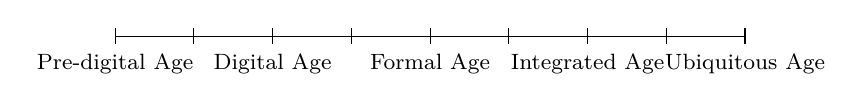
\begin{tikzpicture}
    \draw (0,0) -- (8,0);
    \foreach \x in {0,1,...,8} {
      \draw (\x,-0.1) -- (\x,0.1);
    }
    \foreach \x/\y in {0/Pre-digital Age, 2/Digital Age, 4/Formal Age, 6/Integrated Age, 8/Ubiquitous Age} {
      \node[anchor=north] at (\x,-0.1) {\footnotesize\y};
    }
  \end{tikzpicture}
  \caption{
    Timeline of the ages of data collection.
  }
  \label{fig:collection-history}
\end{figure}

\Cref{fig:collection-history} illutrates the timeline.

\subsubsection{Pre-digital age}

We can consider the earliest records of data collection to be the notches on sticks and
bones to keep tracking of passing of time.  The Lebombo bone, a baboon fibula with
notches, is probably the earliest known mathematical object.  It was found in the Lebombo
Mountains located between South Africa and Eswatini.
They estimate it is more
than 40,000 years old. It is conjectured to be a tally stick, but its exact purpose is
unknown. Its 29 notches suggests that may have been used as a lunar phase counter.
However, since it is broken at one end, the 29 notches may or may not be the total
number\footcite{Beaumont2013}.

Since the early forms of writing, humanity abilities to record events and information
increased significantly.  The first known written records date back to 3,500 BC, the
Sumerian archaic (pre-cuneiform) writing.  This writing system was used to represent
commodities using clay tokens and to record transactions\footcite{Ifrah1998}.

Another important milestone in the history of data collection is the record of
demographic data.  One of first known census was conducted in 3,800 BC in the Babylonian
Empire.  It was ordered to assess the population and resources of
his empire\footcite{Grajalez2013}.

Moving forward many years, I consider a major influential figure in the history of data
collection to be Florence Nightingale (1820 -- 1910).  She was a passionate statistician
and probably the first person to use statistics to influence public and official
opinion.  The meticulous records she kept during the Crimean War
(1853 -- 1856) were the evidence that saved lives.  She was also the first to use
statistical graphics to present data in a way that was easy to understand.  She is
credited with developing a form of the pie chart now known as the polar area
diagram.  She also reformed healthcare in the United Kingdom and
is considered the founder of modern nursing\footcite{Grajalez2013}.

\begin{mainbox}{Florence Nightingale}
  \begin{itemize}
    \item Passionate statistician.
    \item First person to use statistics to influence public and official opinion.
    \item Organized data from garden fruits and vegetables into numerical tables at the age of 9.
    \item At 20 she was receiving two-hour lessons from a Cambridge-trained mathematician.
    \item She found the sight of a long column of figures “perfectly reviving”.
    \item She went out to the Crimean War, to Scutari in Turkey, in 1854.
    \item She found that not even the numbers of soldiers entering the hospitals, or leaving them – alive or dead – was known.
    \item From the first she kept meticulous records.
    \item The data she collected was the evidence that saved lives.
    \item She was the first to use statistical graphics to present data in a way that was easy to understand.
    \item She is credited with developing a form of the pie chart now known as the polar area diagram.
    \item She reformed healthcare in the United Kingdom and is considered the founder of modern nursing.
  \end{itemize}
\end{mainbox}

\subsection{Timeline of data analysis}

\begin{itemize}
  \item Summary statistics
  \item Probability Advent 17, 18th
  \item Statistical learning 19th
    \begin{itemize}
      \item Bayes rule
      \item Gauss’ method of least squares
      \item Playfair data visualization
    \end{itemize}
  \item 20th inference
    \begin{itemize}
      \item Pearson hypothesis testing
      \item Fisher multivariate analysis, maximum likelihood estimate
    \end{itemize}
  \item Computer: McCulloch Pitts, Shannon information theory, Fix and Hodged discriminatory analysis, knn
  \item Machine learning: 1965 Nils Nilsson neural network, 1966 Hunt inducing trees, Kmeans, Vapnik 71
  \item Today: Ensembles, Deep learning: vision and language, KDD
\end{itemize}

\chapter{Preliminaries}
\label{chap:preliminaries}

\chapterprecishere{%
  Maar ik maak steeds wat ik nog niet kan om het te leeren kunnen.\par\raggedleft---
  \textup{Vincent van Gogh}, The Complete Letters of Vincent Van Gogh, Volume Three}

Foundamental concepts in data science come from a variety of fields, including
mathematics, statistics, computer science, optimization theory, and information theory.
This chapter provides a brief overview of the computational, mathematical and statistical
concepts that are used in the rest of the book.

\section{Algorithms and data structures}

Algorithms are step-by-step procedures for solving a problem.  They are used to
manipulate data structures, which are ways of organizing data to solve problems.
They are realized in programming languages, which are formal languages that can be used
to express algorithms.

\subsection{Algoritmic paradigms}

Some techniques are used to solve a wide variety of problems.  They are called
algorithmic paradigms.  The most common ones are listed below.

\paragraph{Divide and conquer}  The problem is divided into smaller subproblems that are
solved recursively.  The solutions to the subproblems are then combined to give a solution
to the original problem.

\paragraph{Dynamic programming}  The problem is divided into overlapping subproblems, and
the solutions to the subproblems are only solved once. The subproblems are then optimized
to find the overall solution.

\paragraph{Greedy algorithms}  The problem is solved with incremental steps, each of which
is locally optimal.  The overall solution is not guaranteed to be optimal.

\subsection{Computational complexity}

Big-O notation, time and space complexity, NP-completeness.

\subsection{Data structures}

Arrays, linked lists, stacks, queues, trees, graphs, hash tables.

\section{Linear algebra}

\subsection{Vectors and matrices}

\subsection{Matrix decompositions}

\textcolor{red}{Verify!}

\paragraph{Singular value decomposition} The singular value decomposition (SVD) of a
matrix $A$ is a factorization of the form
\begin{equation}
  \label{eq:svd}
  A = U \Sigma V^T\text{,}
\end{equation}
where $U$ and $V$ are orthogonal matrices and $\Sigma$ is a diagonal
matrix with non-negative real numbers on the diagonal.  The singular values are the
diagonal entries of $\Sigma$.

\paragraph{Eigenvalue decomposition}  The eigenvalue decomposition of a matrix $A$
is a factorization of the form
\begin{equation}
  \label{eq:eigdec}
  A = Q \Lambda Q^{-1}\text{,}
\end{equation}
where $Q$ is a square matrix whose columns are the eigenvectors of $A$, and
$\Lambda$ is a diagonal matrix whose diagonal entries are the eigenvalues of
$A$.

\paragraph{Cholesky decomposition}  The Cholesky decomposition of a positive-definite
matrix $A$ is a factorization of the form
\begin{equation}
  \label{eq:chol}
  A = L L^T\text{,}
\end{equation}
where $L$ is a lower triangular matrix with real and positive diagonal entries.

\paragraph{QR decomposition}  The QR decomposition of a matrix $A$ is a
factorization of the form
\begin{equation}
  \label{eq:qr}
  A = Q R\text{,}
\end{equation}
where $Q$ is an orthogonal matrix and $R$ is an upper triangular matrix.

\paragraph{LU decomposition}  The LU decomposition of a square matrix $A$ is a
factorization of the form
\begin{equation}
  \label{eq:lu}
  A = L U\text{,}
\end{equation}
where $L$ is a lower triangular matrix with unit diagonal entries and $U$ is
an upper triangular matrix.

\subsection{Eigenvalues and eigenvectors}

An eigenvalue of a square matrix $A$ is a scalar $\lambda$ such that there exists a
non-zero vector $\vec{v}$ satisfying
\begin{equation}
  \label{eq:eig}
  A \vec{v} = \lambda \vec{v}\text{.}
\end{equation}
The vector $\vec{v}$ is called an eigenvector of $A$ corresponding to $\lambda$.

\section{Probability}

\subsection{Axioms of probability}

The Kolmogorov axioms of probability are the foundation of probability theory.
They are
\begin{enumerate}
  \item The probability of an event $E$ is a non-negative real number, i.e. $P(A) \geq 0$;
  \item The probability of the sample space $\Omega$ is one, i.e. $P(\Omega) = 1$; and
  \item The probability of the union of disjoint events, $A \cap B = \emptyset$, is
    the sum of the probabilities of the events, i.e. $P(A \cup B) = P(A) + P(B)$.
\end{enumerate}

\subsection{Permutations and combinations}

\subsection{Conditional probability}

\subsection{Bayes' rule}

\subsection{Independence}

\subsection{Random variables}

\subsection{Probability distributions}

\subsection{Expectation and moments}

\section{Optimization}

\subsection{Minimization of convex functions}

\subsection{Gradient descent}

\subsection{Constraint optimization}

Techniques like Lagrange multipliers, penalty methods, and barrier methods are used to
handle constrained optimization problems in data science.

\subsection{Convex optimization}

Convex optimization problems, where the objective function and the constraints are convex,
have efficient algorithms that guarantee global optimality.

% \subsection{Gradient descent algorithm}
%
% Let $f(\vec{w})$, $f : \mathbb{R}^n \rightarrow \mathbb{R}$, be an objective function that
% we are trying to minimize.  We know that
% $f$ is convex, of class $\mathcal{C}^2$, and its gradient $\nabla f$ is Lipschitz continuous with Lipschitz
% constant $L > 0$.
%
% We want to show that $\lim_{t\rightarrow\infty} f(\vec{w}(t)) = f^{*}$ where $f^{*}$
% is the global minimum of $f$ and $$\vec{w}(t+1) = \vec{w}(t) - \alpha \nabla f(\vec{w}(t))\mbox{,}$$
% for any initial condition $\vec{w}(0)$ and $0 < \alpha \leq \frac{1}{L}$.
%
% Convexity implies that for any two points $\vec{v}$ and $\vec{w}$ in the domain of
% $f$, the line segment connecting them lies above the graph of $f$.  Mathematically, it
% means that $$f(t\vec{v} + (1 - t) \vec{w}) \leq t f(\vec{v}) + (1 - t)
% f(\vec{w})$$ for all $t \in [0, 1]$.
%
% The Lipschitz continuity condition means that the gradient of $f(\vec{w})$ does not change too rapidly.
% Formally, $$\left\|\nabla f(\vec{v}) - \nabla f(\vec{w})\right\| \leq L \|\vec{v} - \vec{w}\|\mbox{,}$$
% for all $\vec{v}$ and $\vec{w}$ in the domain of $f$.  This is a rather weak
% assumption, and it means that the gradient can not change arbitrarily fast.
%
% Since $f$ is convex and twice differentiable, its Hessian is a positive semidefinite
% matrix, and thus its norm is its largest eigenvalue.
%
% A consequence of the Lipschitz continuity for a $\mathcal{C}^2$ function $f$ is that for
% any $\vec{v}$ and $\vec{w}$, we have that
% \begin{equation}
%   \label{eq:lcg1}
%   \vec{v}^T \nabla^2 f(w) \vec{v} \leq L \|v\|^2\text{.}
% \end{equation}
% It means that the eigenvalues of the Hessian are bounded above by $L$.
%
% \paragraph{Descent lemma.}  For $f$, a the multivariate Taylor expansion is that
% $$f(w) = f(v)$$

\chapter{Statistical learning theory}

\chapterprecishere{%
  To  understand  God's  thoughts  we  must study statistics, for these are the measure of His purpose.
  \par\raggedleft--- \textup{Florence Nightingale}, her diary}

We can address several kinds of problems using algorithms that learn from data.  However,
we focus on the problem of \emph{inductive learning}. Before we go further, let us define some terms.

\begin{defbox}{Artificial intelligence}{}
  The field that studies algorithms that exhibit intelligent behavior.
\end{defbox}

Artificial intelligence is a very broad field, including not only the study of algorithms
that exhibit intelligent behavior, but also the study of the behavior of intelligent
systems.  For instance, it encompasses the study of optimization methods, bioinspired algorithms,
robotics, philosophy of mind, and many other topics.  We are interested in the subfield of
artificial intelligence that studies algorithms that exhibit some form of intelligent
behavior.

\begin{defbox}{Machine learning}{}
  The subfield of artificial intelligence that studies algorithms that enable computers to
  automatically learn from data.
\end{defbox}

Machine learning is the subfield of artificial intelligence that studies algorithms that
enable computers to automatically learn and improve their performance on a task from
experience, without being explicitly programmed by a human being.

\begin{defbox}{Predictive learning}{}
  The machine learning paradigm that studies the problem of making predictions given known
  input data.
\end{defbox}

The machine learning paradigm that focuses on making predictions about outcomes (sometimes
about the future) based on historical data. Depending on the reasoning behind the learning
algorithms, the main predictive algorithms are classified in either inductive or
transductive.

\begin{defbox}{Inductive learning}{}
  The machine learning approach that involves deriving general rules from specific
  observations.
\end{defbox}

Induction a type of reasoning that goes from specific instances to more general
principles.  Inductive learning is the machine learning approach that studies algorithms
that, given data representing the set of specific instances, derive general rules that
can make predictions about \emph{any} new instances.

\Cref{fig:learning} give us a hierarchical view of the learning field.  Alternatives ---
such as descriptive learning in opposition to predictive learning, or transductive
learning in opposition to inductive learning --- are out of the scope of this course.

\begin{figurebox}[label=fig:learning]{Organizational chart of the learning field.}
  \centering
  \begin{tikzpicture}
    \draw[outline] (0,0) circle (30mm) node {};
    \node[below] at (0, 2.6) {artificial intelligence};
    \draw[outline] (0,-0.5) circle (25mm) node {};
    \node[below] at (0, 1.6) {machine learning};
    \draw[outline] (0,-1) circle (20mm) node {};
    \node[below] at (0, 0.5) {predictive learning};
    \draw[outline] (0,-1.5) circle (15mm) node {};
    \node[below] at (0, -1.0) {inductive learning};
  \end{tikzpicture}
  % \tcblower
  % Artificial intelligence is a very broad field, including not only the study of
  % algorithms that exhibit intelligent behavior, but also the study of the behavior of
  % intelligent systems.  Machine learning is a subfield of artificial intelligence that
  % studies algorithms that enable computers to automatically learn from data.  A particular
  % case of machine learning is predictive learning, which focuses on making predictions
  % about outcomes given known input data.  Inductive learning is a yet more specific type of
  % learning that involves deriving general rules from specific observations.
\end{figurebox}

Maybe the most general (and useful) framework for predictive learning is Statistical
Learning Theory.  In this chapter, we will introduce the basic concepts of this theory.

\section{Hypothesis}

Consider the set
\begin{equation}
  \label{eq:training-set}
  \big\{(\vec{x}_i, y_i) : i = 1, \dots, n \big\}
\end{equation}
where each sample $i$ is associated with a feature vector $\vec{x}_i \in \mathcal{X}$ and a target variable
$y_i \in \mathcal{Y}$.  We assume that samples are random independent identically
distributed (i.i.d.) observations drawn according to $$P(x, y) = P(x) P(y | x)\text{.}$$
Both $P(x)$ and $P(y|x)$ are fixed but unknown.

This is equivalent to the original learning problem stated by \textcite{Vapnik1995}, where
a generator produce random vectors $\vec{x}$ according to a fixed but unknown
probability distribution $P(x)$ and a supervisor returns an output value $y$ for every
input vector $x$ according to a conditional distribution function $P(y|x)$, also fixed but
unknown.

Moreover, note that this setup is compatible with the idea of tidy data and 3NF (see
\cref{sub:bridge}). Of course, we assume $X, Y$ are only the measured variables (or
non-prime attributes).  In practice, it means that we left aside the keys in the learning
process.

\section{The learning problem}

Consider a \emph{learning machine} capable of generating a set of functions $f(x;
\theta) \equiv f_\theta(x)$, $\theta \in \Theta$ and $f_\theta : \mathcal{X} \rightarrow \mathcal{Y}$.
The problem of learning is that of choosing, among all possible $f_\theta$, the one that
predicts the target variable the best possible way.

In order to learn, we must first define the \emph{loss} (or discrepancy) $\mathcal{L}$
between the response $y$ to a given input $x$, drawn from $P(x, y)$, and the
response provided by the learning machine.

Then, given the \emph{risk function}
\begin{equation}
  \label{eq:risk}
  R(\theta) = \int \mathcal{L}(y, f_\theta(x))\, dP(x, y)\text{,}
\end{equation}
the goal is to find the function $f_\theta$ that minimizes $R(\theta)$
where the only available information is the \emph{training set} \eqref{eq:training-set}.
This is the \emph{empirical risk minimization} (ERM) problem.

This formulation encompasses many specific problems. I focus on the two of them which I
believe are the most fundamental ones: \emph{binary data classification}\footnote{Vapnik
calls it \emph{pattern recognition}.} and \emph{regresssion estimation}\footnote{We are not talking about
\emph{regression analysis}.}.  I left aside the density estimation problem, once it is not
addressed in the remaining of the book.

\paragraph{Binary data classification task.}  In this task, the output $y$ take on
only two possible values, zero or one, and the functions $f_\theta$ are indicator
functions. For the loss
\begin{equation*}
  \mathcal{L}(y, f_\theta(x)) = \begin{cases}
    0 & \text{if } y = f_\theta(x) \\
    1 & \text{if } y \neq f_\theta(x)\text{,}
  \end{cases}
\end{equation*}
we aim at minimizing the risk $\eqref{eq:risk}$ which becomes the probability of
classification error.

\paragraph{Regression estimation task.} Let the outcome $y$ be a real value and
the \emph{regression} $r$ be $$r(x) = \int y\, dP(y|x) \text{.}$$

The regression function is the function $r = f_\theta$ that minimizes the risk function
\eqref{eq:risk} with the loss
\begin{equation*}
  \mathcal{L}(y, f_\theta(x)) = \big(y - f_\theta(x)\big)^2\text{.}
\end{equation*}

\section{ERM inductive principle}

In the following sections, $z$ describes the pair $(x, y)$ and $L(z, \theta)$ a generic loss
function.  The training dataset is thus a set of $n$ i.i.d. samples $z_1, \dots, z_n$.

Since the distribution $P(z)$ is unknown, the risk functional $R(\theta)$ is replaced by
the \emph{empirical risk functional}
\begin{equation}
  \label{eq:empirical-risk}
  R_n(\theta) = \frac{1}{n} \sum_{i=1}^n L(z_i, \theta)\text{.}
\end{equation}

Approximating $R(\theta)$ by the empirical risk functional $R_n(\theta)$ is the so called
ERM inductive principle.  The ERM principle is the basis of the statistical learning
theory.

Classical methods, such as least-squares, maximum likelihood, and maximum a posteriori are
all realizations of the ERM principle for specific loss functions and hypothesis spaces.

In the following sections, we address the four main questions of learning theory.  We
summarize them in \cref{tab:learning-questions}.

\begin{tablebox}[label=tab:learning-questions]{The four main questions of learning theory.}
  \begin{tabularx}{\textwidth}{@{}lX@{}}
    \toprule
    Part & Question \\
    \midrule
    \textbf{Consistency} &
      What are the necessary and sufficient conditions for consistency of a learning process? \\
    \textbf{Rate of convergence} &
      How fast is the rate of convergence of the learning process? \\
    \textbf{Generalization} &
      How can one controle the generalization ability of the learning process? \\
    \textbf{Construction} &
      How can one construct a learning machine that satisfies the conditions of consistency and generalization? \\
    \bottomrule
  \end{tabularx}
\end{tablebox}

\section{Consistency of learning processes}

\section{Rate of convergence of learning processes}

\section{Generalization ability of learning processes}

\section{Construction of learning machines}

\subsection{Data classification methods}

\subsection{Regression estimation methods}

\chapter{Machine learning tasks}

\chapterprecishere{%
  They say ``Na prática, a teoria é outra,'' I say ``Se sua teoria não funciona na
  prática, ela está errada demais.''}

In the previous chapter, we define two fundamental inductive learning tasks:
\emph{classification} and \emph{regression}.  In real-world applications, however, we may
require different tasks to solve our data science problem.  Descriptive learning tasks are
out of the scope of this book, I suggest reading \dots. Even restricting ourselves to
discuss only inductive learning, some machine learning tasks comprise a combination of
fundamental tasks.

Also, we show examples of different inductive biases and how the main learning algorithms
work -- symbolic (decision trees), spatial (nearest neighbors), statistical (naïve Bayes
and Bayesian networks), gradient optimization (neural networks).

\section{Multiclass}

\section{Manifold learning}

\section{Recommender systems}

\section{Reinforcement learning}


\section*{Some examples}

\begin{align*}
 &\vdots\\
 &=12+7 \int_0^2
  \left(
    -\frac{1}{4}\left(e^{-4t_1}+e^{4t_1-8}\right)
  \right)\,dt_1\displaybreak[3]\\
 &= 12-\frac{7}{4}\int_0^2 \left( e^{-4t_1}+e^{4t_1-8} \right)\,dt_1\\
 &\vdots %
\end{align*}

\begin{equation}
  x = a_0 + \frac{1}{\displaystyle a_1
          + \frac{1}{\displaystyle a_2
          + \frac{1}{\displaystyle a_3 + a_4}}}
\end{equation}

\begin{alignat}{2}
 \sigma_1 &= x + y  &\quad \sigma_2 &= \frac{x}{y} \\
 \sigma_1' &= \frac{\partial x + y}{\partial x} & \sigma_2'
    &= \frac{\partial \frac{x}{y}}{\partial x}
\end{alignat}

\fbox{
 \addtolength{\linewidth}{-2\fboxsep}%
 \addtolength{\linewidth}{-2\fboxrule}%
 \begin{minipage}{\linewidth}
  \begin{equation}
   x^2+y^2=z^2
  \end{equation}
 \end{minipage}
}


\[
 \lim_{x\to 0}{\frac{e^x-1}{2x}}
 \overset{\left[\frac{0}{0}\right]}{\underset{\mathrm{H}}{=}}
 \lim_{x\to 0}{\frac{e^x}{2}}={\frac{1}{2}}
\]

\end{document}
